\documentclass[11pt]{paper}

\input{insbox}
\usepackage[x11names]{xcolor}
\usepackage{lineno}

\usepackage{lib/utt-report-template}
\usepackage{lipsum}

\author{Tamas Spisak}
\date{2020}
\newcommand*\mytitle{\color{pniblue}\textbf{'PseudoID'}}

\newcommand*\mysubtitle{\color{pniblue} a pseudonymization system with \\ LimeSurvey integration \\ - dedicated for SFB289 -}

\newcommand*\myshorttitle{PseudoID}
\newcommand*\version{0.1}
\title{\mytitle} % Max 144 chars

\schooltutor{}
\semester{}
\branch{}
\abstracttext{
Pseudonymization is a reversible de-identification process, in which personal data is converted to a pseudonym (ID) that can only be linked again to the personal data by the “pseudonymization entity” (i.e. the single projects in SFB289). The main purpose of pseudonymization is to securely separate experimental from personal data. In clinical research, reversibility is required typically in case of incidental findings.

A proper pseudonymisation protocol can motivate the relaxation, to a certain degree, of data controllers’ legal obligations (if properly applied), i.e. spare a significant amount of efforts put into data security and privacy, when storing, sharing and publishing experimental data \cite{pseudonym}.

Issues of privacy protection constitute a rapidly changing landscape shaped by ongoing digitalization efforts (in general and especially in medical research) and the recent developments in the corresponding regulations (e.g. GDPR). Recent developments render the "traditional" pseudonymization methods typically used in medical reasearch (e.g. the frequently used sequential numbering of participants) increasingly “outdated”, with significant safety concerns (e.g. vulnerability stemming from storing and regularly updating a document linking the personal data to the IDs, or possibility of adversarial re-identification based on the order of data in the pseudonymized dataset).

Here we propose a software tool, called PseudoID, which implements a de-centralized, encryption-based pseudonymization technique which transforms personal data to a pseudonym.
The full of the pseudonym (long ID) allows for complete re-identification (given a dedicated secret digital key, owned by the 'pseudonymization entity', i.e. the individual research site). The software also provides a 'human-readable' short ID (8 characters or barcode), which is easy to link to the long ID and is compatible with most experimental procedures.

PseudoID is equipped with integration to LimeSurvey \cite{limesurvey}, an open-source web application for digital, web-accessible surveys and questionnaires.

\par\noindent\rule{\textwidth\color{pniblue}}{0.4pt}

\textbf{With PseudoID: }
\begin{itemize}
    \item pseudonymization happens as a first step of the experiment, allowing for all succeeding steps to be anonymized;
    \item pseudonyms are deterministic, i.e. reproducible in case of multiple measurements;
    \item pseudonyms are guaranteed (at a pre-defined error level) to be unique for distributed, multi-center experiments of any size;
    \item pseudonymization can be performed at multiple computers/sites simultaneously
    \item pseudonymization happens after a two-factor authentication, and requires a hardware key (or USB stick);
    \item no central administration of the link between pseudonym and personal data is needed
    \item the "pseudonymization secret" is reduced to the (arbitrary number of) USB hardware keys.
\end{itemize}




}

\begin{document}

    %\setlength{\parskip}{0mm}
    %\linenumbers
    \titlespacing*{\section}
    {0pt}{1cm plus 2cm minus 0cm}{0.2cm plus 2cm}
    \titlespacing*{\subsection}
    {0pt}{0.2cm plus 2cm minus 0cm}{0.2cm plus 2cm}

    \frontpage
    
    
    \pagenumbering{arabic}
    \setcounter{page}{2}

    \begin{large}
    \section{Overview of the pseudonymization procedure}
\label{section:overview}
ALIIAS has a number of assumption about the underlying experimental procedures. These assumptions were defined so that they are easy to fit to the majority of medical research experiments. The pseudonymization workflow of SFB289 is illustrated on Fig. \ref{fig:flowchart} and includes the following steps.

\begin{figure}[H]
\centering
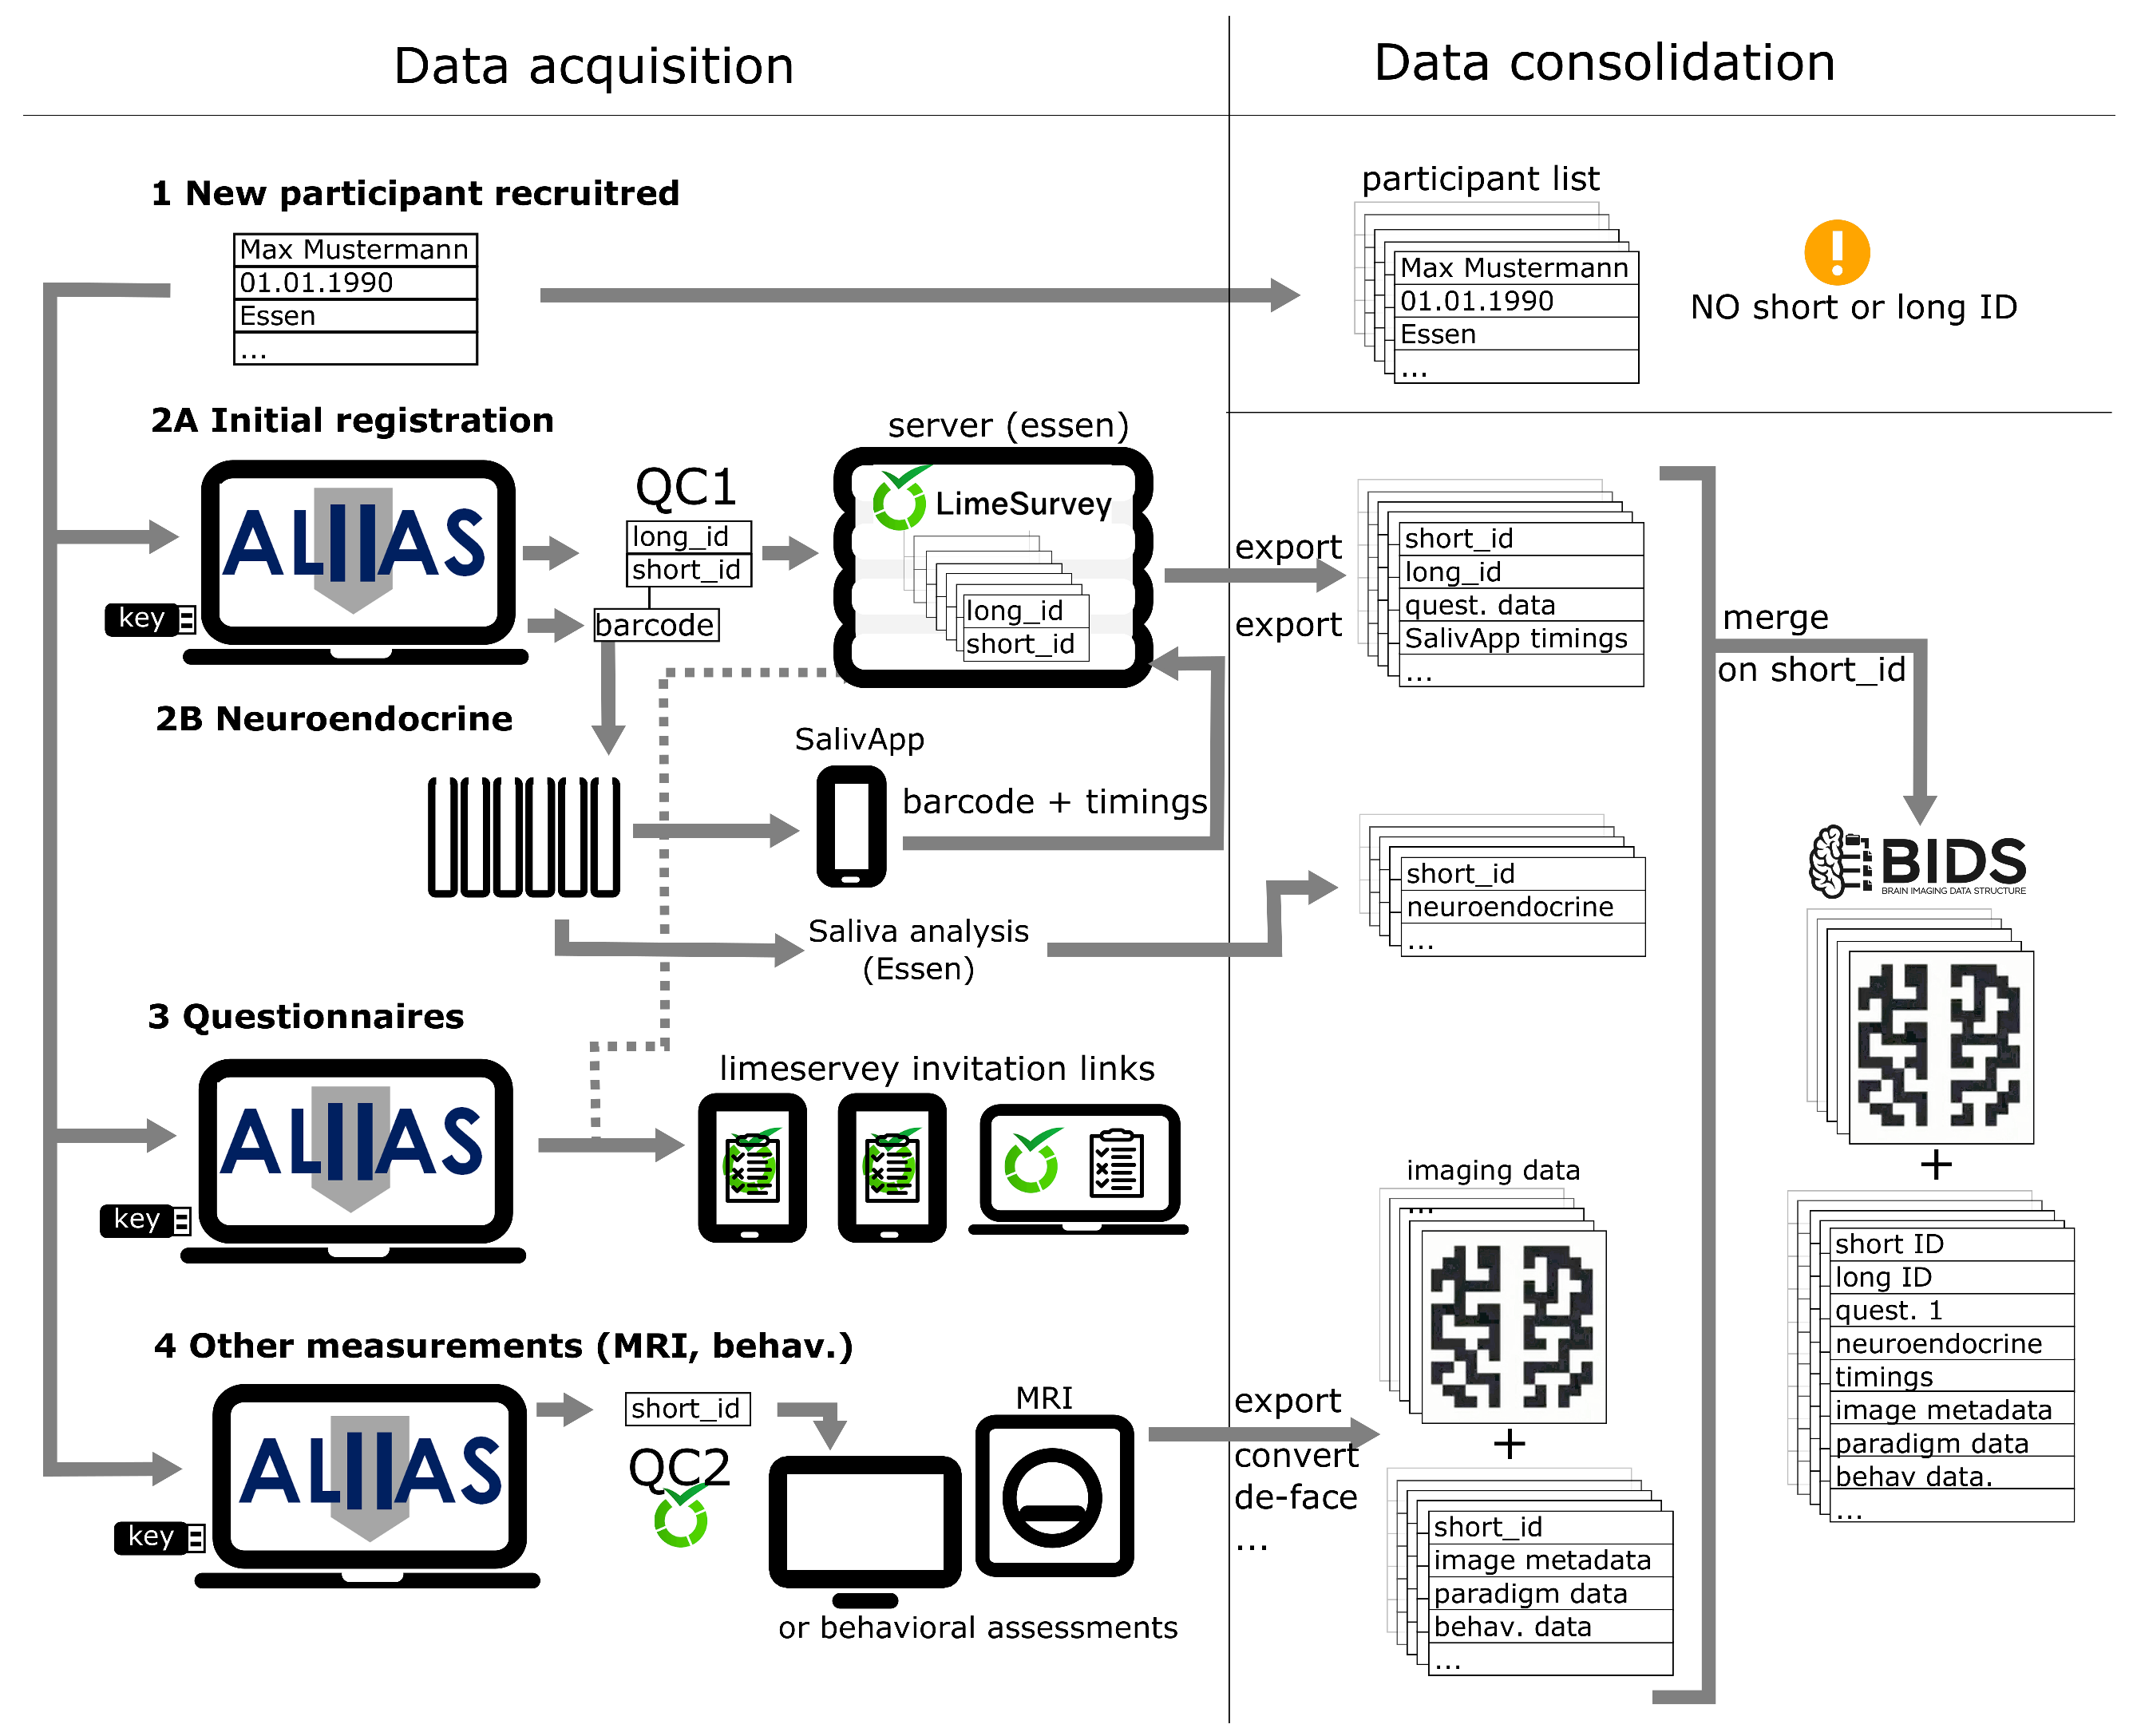
\includegraphics[width=1.0\textwidth]{docs/fig/overview_v3.eps}
\caption{The pseudonymization workflow of SFB289}
\label{fig:flowchart}
\end{figure}

\InsertBoxR{1}{
\small\setlength\fboxsep{5pt}\setlength\fboxrule{1pt}
\fcolorbox{pniblue}{pniblue!5}{\begin{minipage}{0.5\textwidth}
Important Note: the pseudonyms must never be stored in the participant list!
\end{minipage}}
}[1]

\par\noindent\rule{\textwidth\color{pniblue}}{0.4pt}
\textbf{1. Participant recruitment:}
\addcontentsline{toc}{subsubsection}{Participant recruitment}
When a new participant is recruited, his/her personal data and contact details (e.g. address, phone number, e-mail) is recorded on-site (or e.g. during a telephone interview). These data is typically saved into a "participant list" (often an excel table, its maintenance is the responsibility of the single projects, see Fig. \ref{fig:flowchart}). While this participant list itself is also to be protected, ALIIAS is not reliable for the protection of this data. In fact, the main goal of ALIIAS is to make it impossible to link this data to the experimental datasets (unless owning the pseudonymization secret, i.e. the hardware key).
%%\par\noindent\rule{\textwidth\color{pniblue}}{0.4pt}
%\InsertBoxR{-1}{
%\small\setlength\fboxsep{5pt}\setlength\fboxrule{1pt}
%\fcolorbox{pniblue}{pniblue!5}{\begin{minipage}{0.45\textwidth}
%Importantly, even though the web browser is used as a user interface for the software %(thus it looks like a webpage), personal data always stays on the local computer hosting %the software and hardware key.
%\end{minipage}}
%}[1]


\par\noindent\rule{\textwidth\color{pniblue}}{0.4pt}
\addcontentsline{toc}{subsubsection}{Initial registration}
\textbf{2A. Initial registration:} The dedicated hardware key (provided by Z03) is connected to an experimental computer (with ALIIAS already installed) via the USB port. As a next step, the researcher enters the LimeSurvey login credentials in ALIIAS and the provides the following personal data of the participant on the browser interface of ALIIAS (depicted on the left of Fig. \ref{fig:screenshots}):
\begin{itemize}
    \item first name
    \item last name
    \item date of birth
    \item place of birth
    \item mother's maiden name
\end{itemize}

Importantly, even though the web browser is used as a user interface for the software (thus it looks like a webpage), \textbf{personal data always stays on the local computer}, which hosts the software and hardware key.


\begin{figure}[H]
%\centering
\subfigure{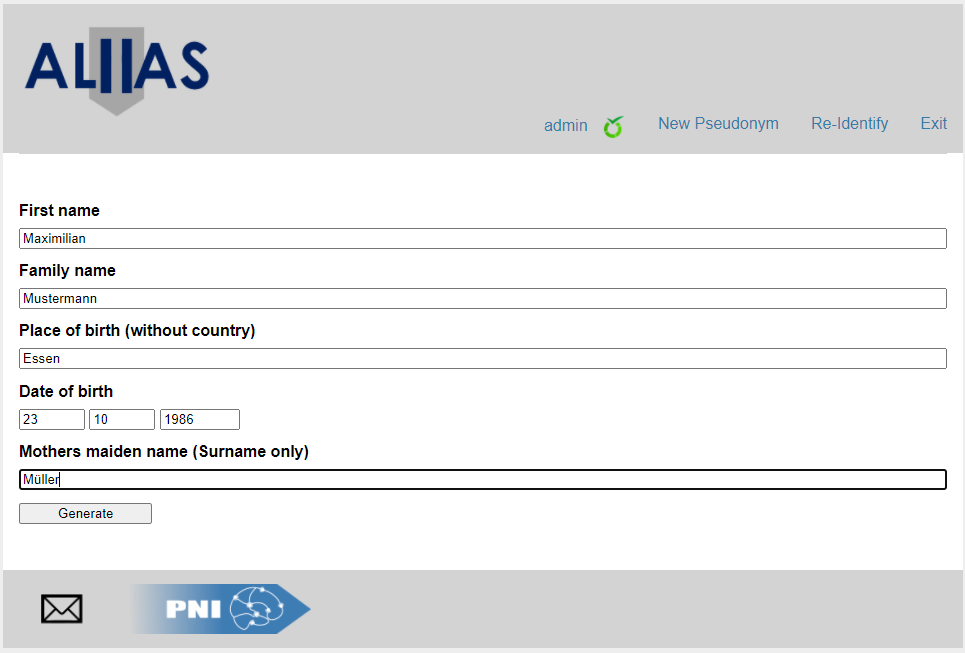
\includegraphics[width=.45\textwidth]{docs/fig/03_filled.PNG}}
\hfill
\subfigure{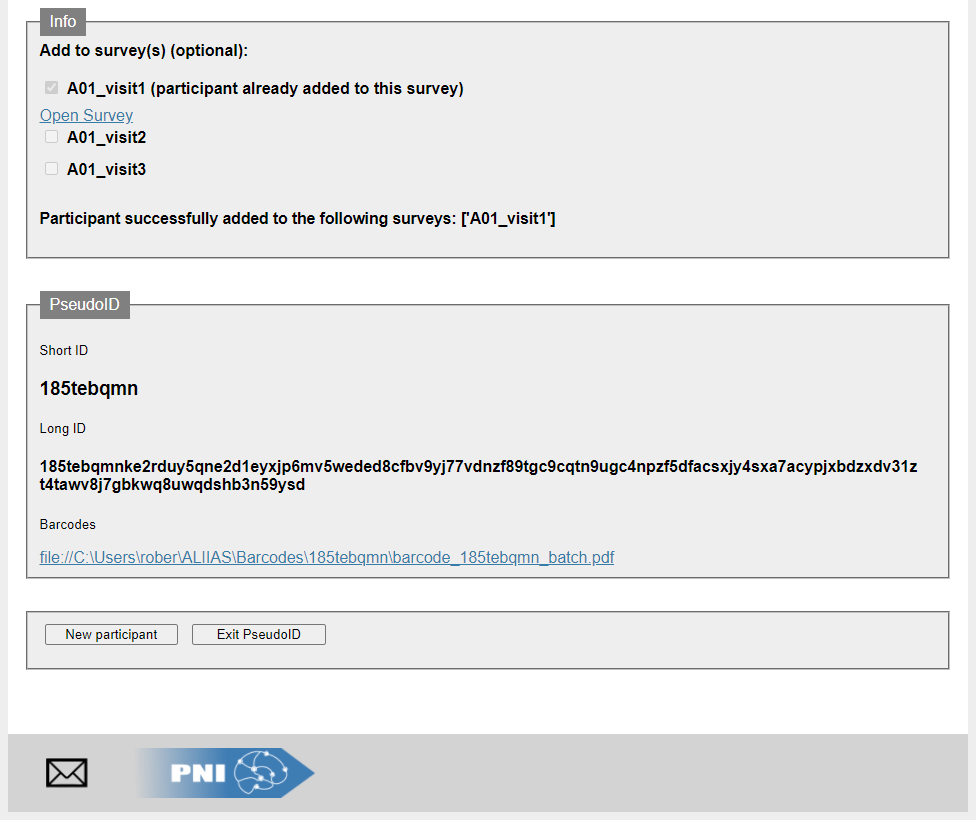
\includegraphics[width=.45\textwidth]{docs/fig/05_pseudonym.PNG}}
\caption{The browser-based user interface of ALIIAS.}
\label{fig:screenshots}
\end{figure}

ALIIAS reads the "pseudonymization secret" from the hardware key and uses it to generate pseudonym. After the user confirms that the data is correct, the software outputs the long and short-version of the pseudonym (on the right of Fig. \ref{fig:screenshots}). Both the long and short IDs are unique for the whole CRC. De-identification is only possible with the long-id. During the initial registration, ALIIAS automatically connects to the LimeSurvey server hosted at the University Duisburg-Essen and registers the participant's long and short IDs to any of the surveys belonging to the single project. Additionally, ALIIAS converts the short ID into a barcode (see step 5) for labelling assessment tools belonging to the participant.

\par\noindent\rule{\textwidth\color{pniblue}}{0.4pt} 
\addcontentsline{toc}{subsubsection}{Compatibility with neuroendocrine and genetic assessments}
\textbf{2B. Compatibility with neuroendocrine and genetic assessment and Biobank:} Upon the initial registration, ALIIAS generates a set of barcodes, encoding the short ID. These will be printed by the barcode printers provided by the central projects and used to label the saliva sampling kit (+ genetics) for the given participant (refer to the corresponding SOP of Z02). These barcode labels will be scanned by the participant, using the dedicated smartphone application of SFB289 (SalivApp), directly after during sample collection (for precise timing). The ShortID encoded in the barcode is obtained in Z02 to link saliva sample results with sample timings, genetics and BioBank-IDs.

\par\noindent\rule{\textwidth\color{pniblue}}{0.4pt}
\addcontentsline{toc}{subsubsection}{Questionnaires}
\textbf{3. Questionnaires:}
 In SFB289, questionnaire data will be collected with LimeSurvey. After the participant has been assigned to a survey, ALIIAS provides an individualized invitation link, which can be opened in another browser tab or e-mailed to the participant. Questionnaires can be filled in on any computer (or tablet), with internet connection. 
 If the initial registration and the assignment of the participant to a given questionnaire take place in different time points (e.g repeated measures), ALIIAS can be used again and again to obtain the (permanent) short ID of the participant, given his/her personal data (either from the local 'participant list', see step 1., or as provided by the participant.
 Multiple assessment points (repeated measures) are handled as separate surveys in LimeSurvey (refer to section \ref{section:ls_setup} for more details).
 
 \par\noindent\rule{\textwidth\color{pniblue}}{0.4pt}
 \addcontentsline{toc}{subsubsection}{Other measurements}
 \textbf{4. Other measurements (MRI, behavior):}
 For other measurements, ALIIAS can be used repeatedly to obtain the shortID of the participant (given the hardware key). The short ID can than be used in the dedicated experimental system (e.g. the MRI console) as the identifier ("name") of the participant, so that it gets exported together with the experimental data. In case of repeated measurements, ALIIAS is simply used multiple times to obtain the short ID. Single projects can add arbitrary "experimental tags" to the short ID (e.g. append '-w2' for week 2) or use the built in features of the given experimental equipment (e.g. separate 'program cards' on the MRI console) to distinguish between measurements.

\par\noindent\rule{\textwidth\color{pniblue}}{0.4pt}
\addcontentsline{toc}{subsubsection}{Data Consolidation and re-identification}
\textbf{Data Consolidation and re-identification:} The experimental data (either exported form the LimeSurvey database, or via the dedicated experimental systems) - if required - will be subject of further anonymization (e.g. de-facing of structural MRI images) The central scientific project will provide recommendations and share software tools for these tasks. Merging of experimental data from different sources or different assessment points is based on the short ID. The LimeSurvey database provides the link between the short and long IDs. The latter can be used for re-identification, e.g. in case of incidental findings by the owners of the hardware key.
    %\par\noindent\rule{\textwidth\color{pniblue}}{0.4pt}
\section{Example use-cases}
\label{use-case:one-session}
\par\noindent\rule{\textwidth\color{pniblue}}{0.4pt}
 \addcontentsline{toc}{subsubsection}{Single-session}
\textbf{1. Initial registration only (single-session use-case):}
If questionnaires are the only type of data collected or all assessments (e.g. questionnaires + behavioral experiment) are done in one session (i.e with starting ALIIAS once, for pseudonymization of one participant), the initial registration with ALIIAS might already be sufficient. The researcher can instantly obtain the invitation link to the survey an the obtained short ID can be used for subsequent assessments, directly following the initial registration.

\par\noindent\rule{\textwidth\color{pniblue}}{0.4pt}
\addcontentsline{toc}{subsubsection}{Multi-session}
\textbf{2. "Batched" initial registration of many subjects (multi-session use-case):}
With the proposed pseudonymization procedure, the researcher has the opportunity to "batch" initial registrations, i.e. perform the initial registration of many participants in one longer session, based on the personal data previously collected (e.g. during phone interview). The assignment of the participants to specific surveys and the actual experiments (MRI, behavior) can take place at a later time point. In this case, ALIIAS can be used multiple times to repeatedly obtain the pseudonym for a given participant. ALIIAS displays if the participant was previously registered to any of the surveys. If the experimenter has previously registered the participant, this feature can be used for error checking. (Typographical errors in the personal data result in a different pseudonym which has not been registered yet, see ).

\par\noindent\rule{\textwidth\color{pniblue}}{0.4pt}
 \addcontentsline{toc}{subsubsection}{Repeated measures}
\textbf{3. Repeated assessments (multi-session + repeated measures use-case):}
Use-case 2 is easy to adapt to repeated assessments (e.g. before and after treatment). Single projects can add arbitrary ”experimental tags” to the shortID (e.g. append ’-w2’ for 'week 2') or use the built in features of the given experimental equipment (e.g. separate ’program cards’ on the MRI console) to distinguish between measurements. 

\par\noindent\rule{\textwidth\color{pniblue}}{0.4pt}
 \addcontentsline{toc}{subsubsection}{Parallel-sessions}
\textbf{4. Simultaneous assessment of many subjects (parallel-sessions use-case):}
PseudoID can be run on multiple computers simultaneously without any further notice. The reproducibility and uniqueness of pseudonyms and the consistency of the LimeSurvey database are still guaranteed.

\par\noindent\rule{\textwidth\color{pniblue}}{0.4pt}
\addcontentsline{toc}{subsubsection}{Computer failure during session}
\textbf{5. Computer failure during experiment:}
If the experiment has to be restarted, PseudoID can be repeatedly used to obtain the short ID. In the case of failure of the computer on which PseudoID runs, a backup computer can be used to obtain the short ID (even if the initial registration and other pseudonymization sessions were not performed on that computer).

\par\noindent\rule{\textwidth\color{pniblue}}{0.4pt}
\addcontentsline{toc}{subsubsection}{Incidental finding}
\textbf{6. Incidental finding:} In case of incidental finding, the LimeSurvey database will be used to link the long ID to the short ID and re-identification is performed by PseudoID (on any computer), given the long ID and the pseudonymization secret stored on the hardware key. 

\par\noindent\rule{\textwidth\color{pniblue}}{0.4pt}
\section{Quality Checks}
\label{section:qc}
Typographical errors in the personal data will result in a different pseudonym. This might not be a serious problem if the pseudonym is obtained only once as, in this case, re-identification of this pseudonym will simply result in the mistyped personal data. (Use case \ref{use-case:one-session}).
However, if ALIIAS is used for obtaining the pseudonym for the same subject multiple times (Use cases 2,3 and 5), typographical errors result in different pseudonyms for the same subject which requires manual adjustment during data consolidation.
To avoid this, two quality check steps must to be performed.
\begin{itemize}
    \item \textbf{QC1:} Typographical are most critical at the initial registration. Therefore, before displaying the pseudonym, ALIIAS shows a preview page, where personal data must be carefully checked for mistakes. Note, that ALIIAS automatically converts some characters which might be source of ambiguity (Table \ref{tab:typo}). The researcher must explicitly state that "All details are correct", before being able to obtain the pseudonym (see label 'QC1' on Fig. \ref{fig:flowchart}).
    \item \textbf{QC2:} If the initial registration was correct and the researcher already assigned the participant to at least one survey in ALIIAS (recommended to do right at initial registration), than at repeated pseudonymization of the same participant, the preview page of ALIIAS will display the surveys to which the participant was already assigned. This feature can be considered as a additional opportunity for quality checking: in case of typos the researcher will see result contradictory to the expectations. Namely, ALIIAS will display that no participant with the (mistyped) details was added to any of the surveys.
\end{itemize}

\begin{table}[h]
 \caption{Handling of potentially ambiguous characters in ALIIAS}
  \centering
  \begin{tabular}{l l}
    \toprule
    Input Character      & Automatically converted to      \\
    \midrule
    \midrule
    ä            & ae                 \\
    \midrule
    ü           & ue                \\
    \midrule
    ö           & oe                \\
    \midrule
    ß           & ss                \\
    \midrule
    whitespace          &              \\
    \_          &              \\
    ,          & omitted             \\
    (          &              \\
    )          &              \\
    .          &              \\
    \bottomrule
  \end{tabular}
  \label{tab:typo}
\end{table}

    \section{Installation}
PseudoID is designed to be installed on Windows computers and requires administrator privileges (i.e authorization from the IT department, for each installation individually).

\begin{itemize}
    \item Click \href{https://github.com/spisakt/PseudoID/releases}{\underline{here}} to access the latest version of PseudoID.
    \item Download the following files to an arbitrary folder\footnote{If you can not see the file extensions, you should activate them under "View" in the explorer}: 
    \begin{itemize}
        \item \path{start_pseudoid.exe}
        \item \path{pseudoid.txt}
        \item \path{handler.txt}
        \item \path{settings.conf} 
    \end{itemize}
    \item If you have administrator privileges on the computer, simply double-click the file called \path{start_pseudoid.exe} to start the software.
    
    Refer to the instructions below if you are working on a centrally administered computer.
\end{itemize} 

\subsection*{Installation on centrally-administered computers}

Please contact the IT department (via phone call or ticket) and ask for privileges for running the software. Explain the IT department what the software exactly does: "PseudoID is a research software for SFB289. Technical details: it is a flask application deployed as a standalone exe file. It reads two configuration files from the same folder and runs a webserver on the localhost (Port 5000)".

As an additional information. you can provide the following steps, which worked at the University Hospital Essen.

\begin{enumerate}
    
    \item The administrator from the IT department should move \path{start_pseudoid.exe}, \path{handler.txt} and \path{settings.conf} to a directory, from which the \path{.exe} can be executed. Caution: They have to be in the SAME folder. 
    
    \item The \path{pseudoid.txt} file should be moved to a location that can be accessed by the user, for example the desktop. The file should then be opened with the basic text editor, to change the current path to the path where the \path{.exe} was moved to
    \label{item:admin}
    
    \item For example: the current \path{pseudoid.txt} ends like this: \\ \path{.\pseudoid.exe}. \\ This should be changed to the NEW path of the \path{start_pseudoid.exe}
    
    \item When this has been changed correctly, the file name of \path{pseudoid.txt} has to be changed to \path{start_pseudoid.bat} (you can ignore the warning)
    
    \item If everything worked out properly, a double-click on \path{start_pseudoid.bat} should start PseudoID in a new browser window!
    
    \item The command line window can be closed, when PseudoID is closed.
\end{enumerate} 



    \section{Developers and Acknowledgement}
PseudoID was developed by Tamas Spisak and Robert Englert (PNI-lab, University Hospital Essen). The proposed pseudonymization workflow is a result of a joint effort of members of the central scientific projects of SFB289 (Ulrike Bingel, Christian Büchel, Winfried Rief, Manfred Schedlowski and Tamas Spisak) and implements insights from several PIs of SFB289.
        
    \end{large}

    %\nocite{*}
    \bibliographystyle{apalike}
    \footnotesize
    {\linespread{0}\selectfont\bibliography{references}}
\end{document}
